\section{Methods}\label{sec:method}
The goal is to adapt a pretrained VLA to complete language-conditioned manipulation tasks on a target robot. The policy receives camera images, proprioception, and an instruction, predicts an action chunk, and executes a prefix before observing again. We evaluate complete-task success independently of the reward used for training.

During acquisition, each skill has its own instruction, success condition, and starting states. For example, placement can begin with an object already held. During composition and final evaluation, the robot starts with an empty gripper and receives one complete-task instruction. This distinction prevents isolated skill performance from being treated as full-task success.


\subsection{Dense Acquisition, Binary Refinement, and Self-Imitation}
We first train approach, pickup, and placement skills with dense rewards. Distance reduction and manipulation events guide exploration before skill success becomes common. After dense acquisition, we refine the skills using binary success rewards.

Successful trajectories are retained by instruction. When later training degrades earlier skills, self-imitation fits a balanced mixture of earlier and current successes:
\begin{equation}
\mathcal L_{\rm SI}=\mathbb E_{\rm success}
\left[\|\hat a-a\|^2\right].
\label{eq:si_loss}
\end{equation}
Here $\hat a$ is the predicted action and $a$ is the recorded executed action. The average balances instructions and excludes unused action slots. Policy-dependent features are refreshed before fitting. Balancing matters because imitating only the newest skill can reinforce forgetting.

Algorithm~\ref{alg:paper_pipeline} summarizes the schedule. Progress is checked with fixed skill evaluations. After an initial training period, automated stages can end at a success target or a plateau; budget exhaustion also ends a stage. The CDPR sequence used validation-guided manual transitions. After consolidation, all learned skills are evaluated again. Automated runs retain the consolidation update only when recovery improves the degraded skills on average and keeps other skills within tolerance.
% Method-level schedule. Automatic stopping is implemented for WX200;
% the historical CDPR sequence used validation-guided manual transitions.
\begin{algorithm}[!t]
\caption{Staged VLA adaptation}
\label{alg:paper_pipeline}
\small
\begin{algorithmic}[1]
\Require Pretrained VLA, skill instructions, fixed evaluations
\State Initialize the target action controller and success banks
\For{reward mode: dense acquisition, then binary refinement}
    \For{skill: approach, pickup, placement}
        \Repeat
            \State Collect same-scene rollout groups for the skill
            \State Update with $\mathcal L_{\rm RL}$; retain successful trajectories
            \State Evaluate skill success
        \Until{target, plateau, or stage budget ends training}
        \State Evaluate retention of all learned skills
        \If{earlier skills have degraded}
            \State Balance earlier and current successful experience
            \State Fit $\mathcal L_{\rm SI}$; validate recovery and retention
        \EndIf
    \EndFor
\EndFor
\Repeat
    \State Collect full-task rollouts from empty-gripper starts
    \State Assign milestone credit; protect achieved prefix skills
    \State Update with $\mathcal L_{\rm RL}$; evaluate complete-task success
\Until{target, plateau, or full-task budget ends training}
\State \Return One policy for the complete instruction
\end{algorithmic}
\end{algorithm}


\subsection{SmolVLA with an Embodiment-Specific Residual}
Figure~\ref{fig:architecture} shows one implementation of the pipeline. Following the residual-learning ingredient of Probe, Learn, Distill (PLD)~\cite{pld}, we retain a pretrained expert and adapt its actions with a lightweight residual. The SmolVLA expert supplies an action prior, mapped to the target control interface. In our five-channel controller, eight action slots form a 40-dimensional prior.
A frozen visual projection supplies 512 features; six proprioceptive values complete the 518-dimensional observation. The residual receives this observation and the 40-dimensional prior, and predicts a bounded correction. The combined action is bounded before execution.

LoRA adapts the action expert during earlier training. In the evaluated full-task continuation, the inherited VLA and LoRA weights are frozen while the residual and exploration parameters are trained. The backbone, action mapping, and feature dimensions can change with the embodiment; the training schedule remains the same.

\begin{figure*}[!t]
\centering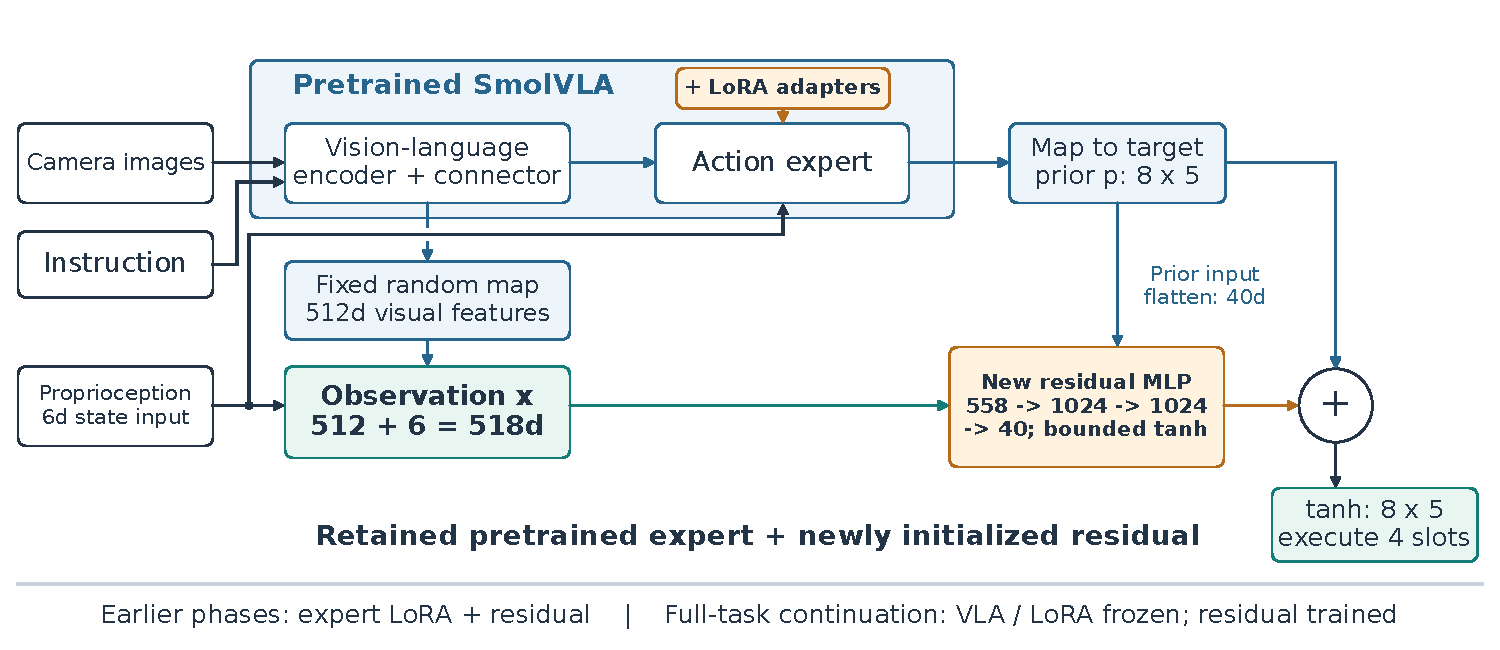
\includegraphics[width=\textwidth]{figures/smolvla_residual_lora.pdf}
\caption{SmolVLA implementation of the pipeline. The added residual combines 518 observation features with a 40-dimensional action prior. LoRA adapts the pretrained expert during earlier training; the evaluated full-task continuation freezes the VLA and LoRA weights. Feature and action dimensions refer to the five-channel controller.}
\label{fig:architecture}
\end{figure*}

\subsection{Milestone-Based Full-Task Composition}
After skill consolidation, one policy learns the complete instruction from empty-gripper starts. No external controller switches between specialist policies. Approach, held pickup, and final placement serve as milestones for assigning credit within a rollout.

The main rule is simple: a later placement failure should not remove the local credit for a successful approach or pickup. We compare milestone outcomes within groups of rollouts from the same scene. Actions receive credit for the milestone they contribute to, while full-task success provides an additional preference for completing the chain. A negative completion bonus is suppressed on already achieved approach and pickup milestones. Placement receives its completion credit once.

This rule preserves useful partial behavior while training the remaining task. It controls the assigned credit; it does not prevent interference through shared network parameters.

\subsection{Stabilized Updates and Full-Task Continuation}\label{sec:rl_loss}
We use a clipped group-relative policy loss with entropy regularization:
\begin{equation}
\mathcal L_{\rm RL}=\mathcal L_{\rm clip}-\eta\mathcal H.
\label{eq:rl_loss}
\end{equation}
The clipped loss compares rollouts within each scene group and limits the incentive for large changes in action likelihood. We use separate upper and lower clipping bounds. The entropy term $\mathcal H$, weighted by $\eta$, maintains exploration during manipulation and composition. Together, these choices help keep early updates conservative while successful behavior is still rare.

During skill learning, DAPO-style dynamic sampling filters uninformative groups and collects additional rollout groups within the configured collection budget~\cite{dapo}. With binary rewards, uniform outcomes provide no group-relative contrast. During dense acquisition, filtering instead checks within-group return variation, so partial progress can provide a learning signal before a group contains a successful skill execution.

The CDPR continuation starts from a full-task plateau. It retains the learned residual, freezes the inherited VLA and LoRA, and starts a fresh optimizer with the same milestone rewards. It also corrects how sampled actions are scored during policy updates.

Policy-gradient updates compare how likely a recorded sample is under the old and new policies. For a Gaussian policy followed by clipping, an established approach uses the original sample for this calculation~\cite{capg}. For example, sampled commands of 1.2 and 1.8 both become 1.0 after clipping; retaining the original value identifies which sample was drawn.

Our earlier CDPR implementation evaluated the clipped command under a Gaussian density. It also treated an exploration offset shared across an episode as independent additional noise at each decision. The continuation stores both the original sample and the applied offset. Old and new policy likelihoods then score that same sample with the same recorded offset. This makes the likelihood calculation consistent with the sampling process.

Concretely, let $\mu_{\theta,t}$ be the bounded residual controller's predicted mean and $\sigma_\theta$ its learned exploration scale. An offset is sampled once per episode and applied during selected phases; $b_t$ records its applied value at decision $t$. Sampling and execution are
\begin{equation}
\begin{aligned}
u_t&\sim\mathcal N(\mu_{\theta,t}+b_t,\operatorname{diag}(\sigma_\theta^2)),\\
a_t&=\operatorname{clip}(u_t,-1,1).
\end{aligned}
\label{eq:latent_action}
\end{equation}
The robot executes $a_t$; the likelihood ratio uses the stored $u_t$ conditional on $b_t$. The residual and exploration scale remain trainable. Section~\ref{sec:cdpr_results} reports the resulting full-task continuation, whose endpoint does not isolate the effect of this likelihood correction.

\subsection{Intermediate Feedback for LIBERO Composition}\label{sec:dense_method}
The LIBERO study asks whether intermediate feedback remains useful when a pretrained policy already performs manipulation skills. We fine-tune an OpenVLA-OFT-based policy with SimpleVLA-RL and LoRA on complete LIBERO-Spatial instructions~\cite{openvlaoft,simplevlarl,libero}. This tests the feedback component of the approach when a conventional robot action interface is already available.

We compare terminal-only reward, phase rewards for completed subgoals, and dense feedback that also resolves progress within a phase. A tracker follows reach, grasp, lift, move, and place. Within the active phase, dense credit is given only when progress exceeds its previous maximum; revisiting the same position earns no repeated credit. The progress baseline resets at each phase transition.

Shaping is bounded and added to the terminal reward, while the native task-success verifier remains unchanged. Optional filtering selects rollout groups by their fraction of terminal successes, independently of shaping. We evaluate both the full suite and a separate low-success task (Section~\ref{sec:libero_results}). These comparisons test whether progress feedback helps compose available skills under one instruction, as well as supporting learning when terminal success is rare.

The motivation follows from a simple group calculation. For $G$ independent rollouts from one scene, each with success probability $p$, the probability of observing both success and failure is
\begin{equation}
P_{\rm mixed}=1-p^G-(1-p)^G.
\label{eq:mixed}
\end{equation}
With eight rollouts, this probability is only 21.6\% at 3\% success, but 94.2\% at 30\% success. Milestones can therefore provide informative comparisons before complete-task success becomes common. Dense feedback can also distinguish all-failure rollouts. A filter that removes such groups discards this potential signal.

